\chapter{Метод термостимульованих струмів}\label{chapTSC}

Метод термостимульованих струмів
(thermally stimulated current, TSC)
спирається на вивчення температурної залежності струму для зразка,
у якому попередньо створено нерівноважних (надлишковий) розподіл зарядів, захоплених на дефектах.
Найчастіше подібне збудження зразка реалізується внаслідок освітлення
у видимому діапазоні чи завдяки інжекції носіїв з контактів,
за допомогою яких потім вимірюється струм.
Проте використовується також збудження завдяки опроміненню
рентгенівськими чи гамма-квантами, електронними чи позитронними пучками,
$\alpha$--частинками, нейтронами.

Як правило, щоб сповільнити процеси емітування дефектами захоплених носіїв,
дослідження проводяться у температурному діапазоні,
нижня границя якого $T_0$ досягає азотних або й гелієвих температур.
При цьому збудження може відбуватися як під час всього процесу попереднього охолодження,
так і лише при знижених температурах.
Якщо збудження інжекційне, то в першому випадку застосовують
термін TSC дополяризації, а  в другому --- TSC поляризації.

Режим нагрівання схожий на той, що
використовується при ізохронному відпалі, тобто відбувається з постійною
швидкістю:
\begin{equation}
\label{TSCT}
T(t)=T_0+a_T\,t\,.
\end{equation}
Величина коефіцієнта $a_T$ зазвичай невелика,
декілька кельвінів на секунду, щоб
можна було знехтувати градієнтом температури у зразку.
Нагрівання відбувається при постійній електрична напрузі (або напруженості електричного поля).

Загалом, електричний струм має дві складові:
пов'язану з власною провідністю та викликану релаксацію захоплених зарядів.
Друга і є власне термостимульованим струмом $I_{TS}$, який потрібно виокремити з експериментальних результатів,
використовуючи відому температурну залежність першої компоненти.
ЇЇ, наприклад, можна отримати проводячи попередні вимірювання незбудженого зразка.

\begin{figure}[t]
\center
\vspace{-2mm}
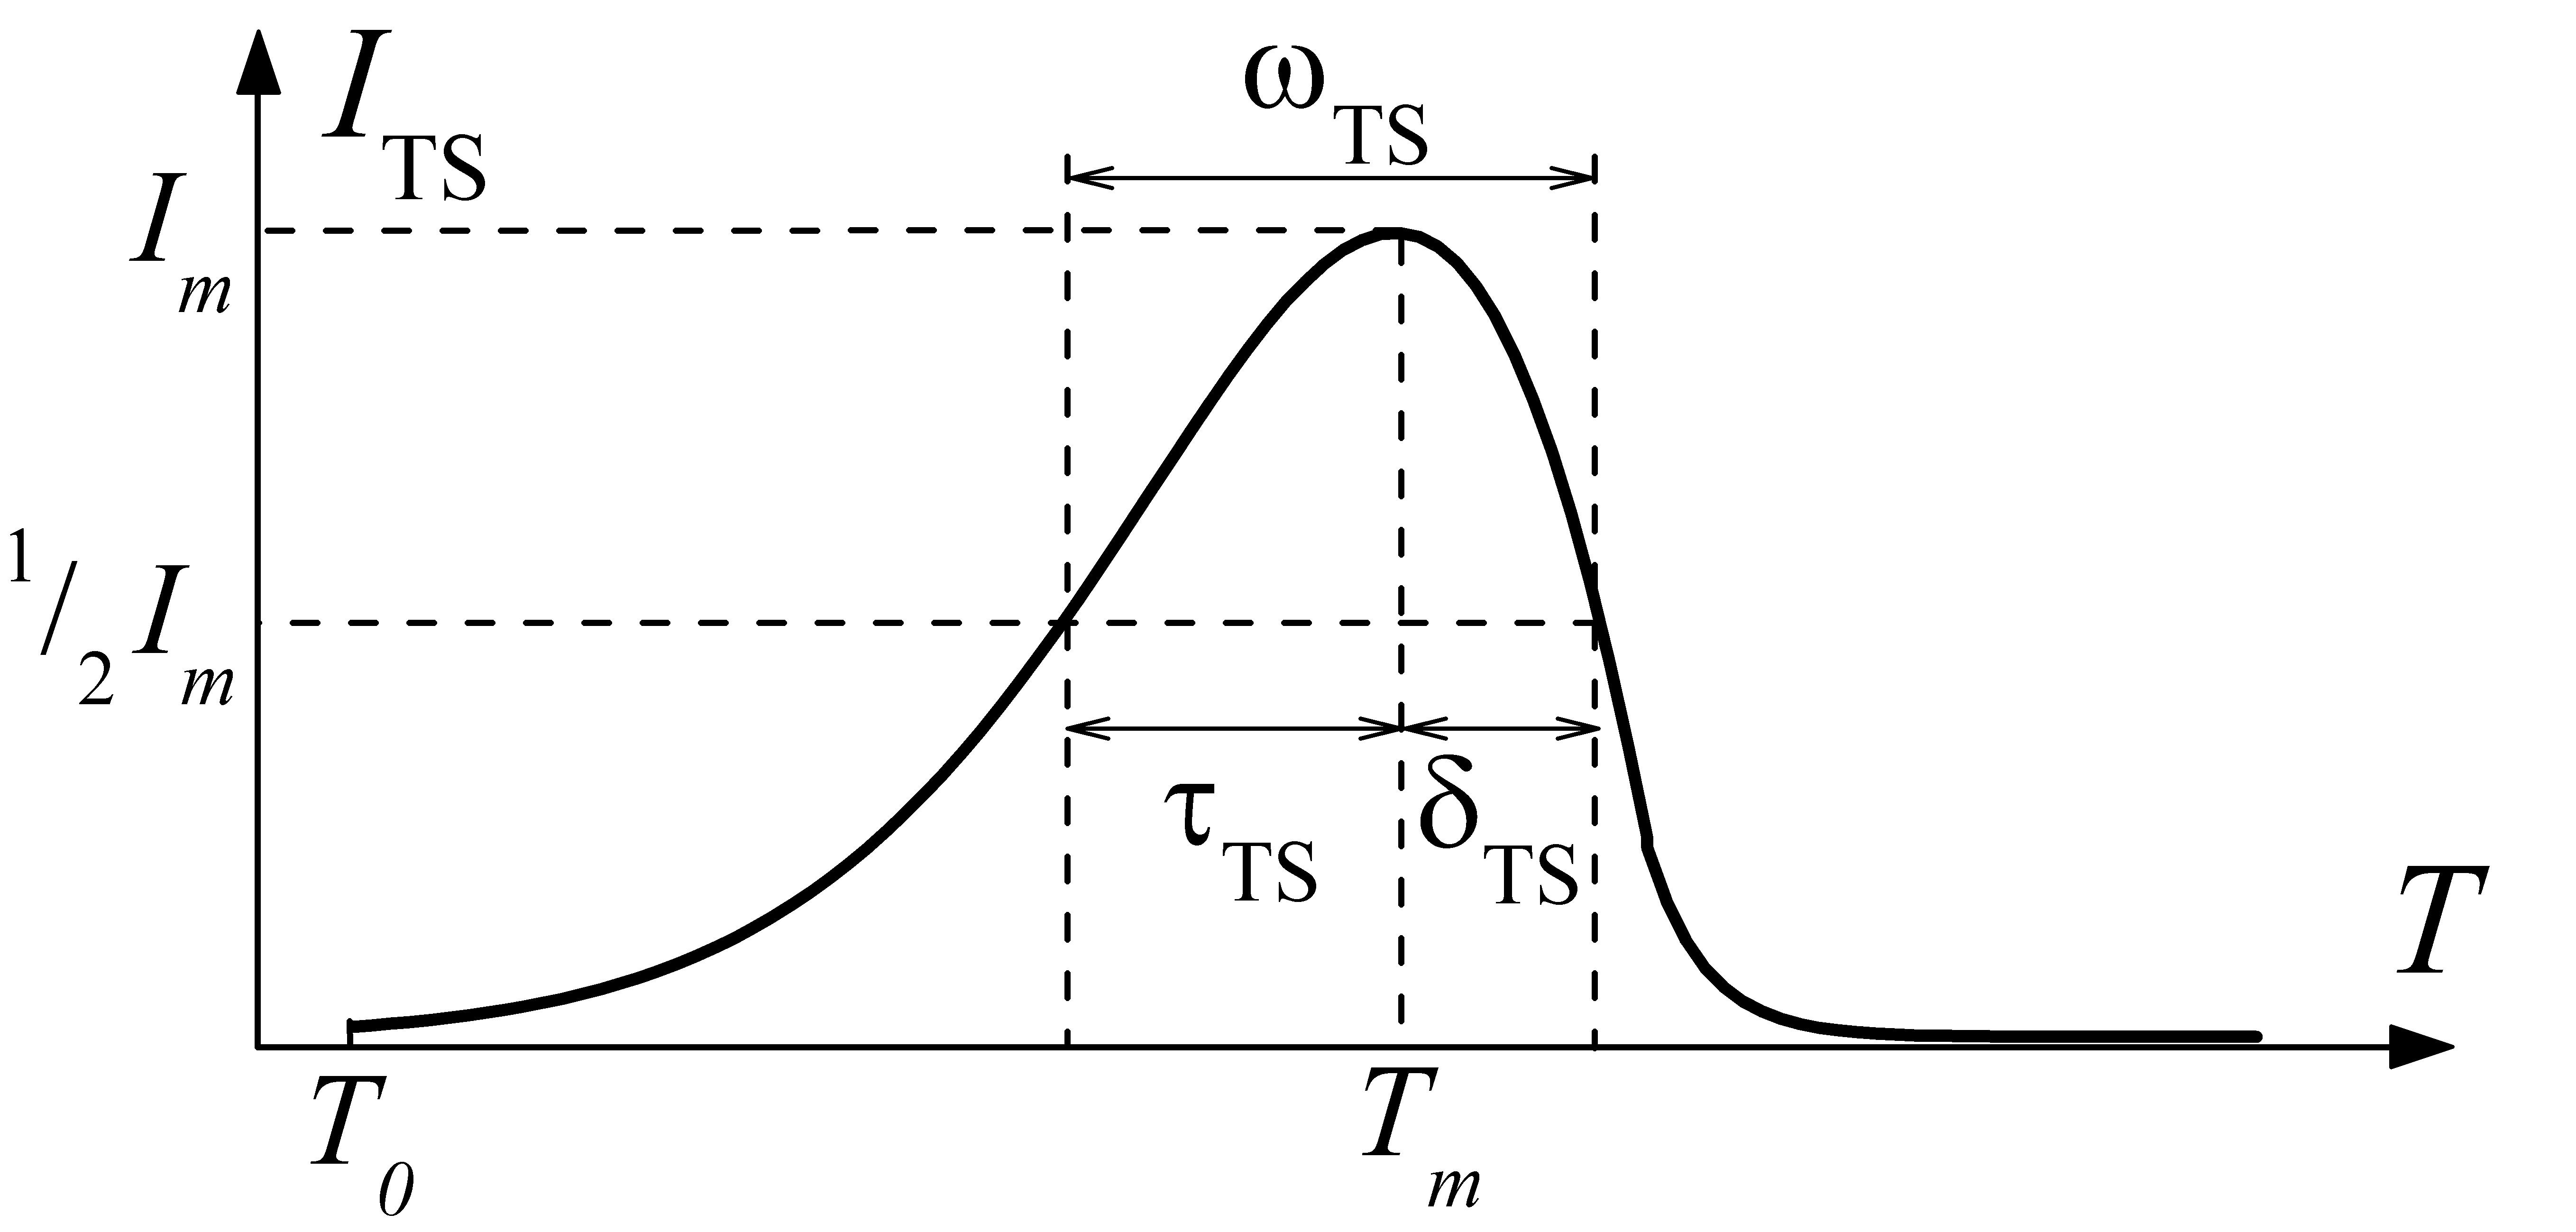
\includegraphics[width=0.7\textwidth]{Fig4_1}
\vspace{-3mm}
\caption{Типовий сигнал термостимульваного струму
за наявності пасток одного типу.}
\vspace{-3mm}
\label{F41}
\end{figure}

У випадку наявності одного типу пасток залежність $I_{TS}(T)$ має вигляд
несиметричного дзвону (див. рис.~\ref{F41}),
причому для температури максимуму цієї залежності виконується співвідношення
\begin{equation}
\label{TSCTm}
\frac{E_C-E_t}{kT_m^2}=\frac{e_n}{a_T}=\frac{\sigma_n\,\upsilon_{th,n}\gamma_g N_C}{a_T}\exp\left(-\frac{E_C-E_t}{kT_m}\right)\,.
\end{equation}
Вираз (\ref{TSCTm}) записано у припущенні, що наявна пастка захоплює переважно електрони;
при цьому використано формулу (\ref{en}).

Для визначення енергетичного положення рівня, пов'язаного з дефектом застосовують декілька підходів.
А саме.

У методі зсуву максимуму проводять вимірювання при декількох швидкостях нагріву.
При цьому положення $T_m$ також буде зміщуватися по температурній шкалі, що
дозволяє отримати декілька рівнянь на кшталт (\ref{TSCTm}) ---
підхід, схожий на той, що використовується у традиційній DLTS.

Метод напівширин передбачає, що має бути відомою температурна залежність
множника, розташованого перед експонентою у виразі (\ref{TSCTm}):
$(\sigma_n\,\upsilon_{th,n}\gamma_g N_C)\sim T^{\alpha_{\mathrm{TS}}}$.
Фактично, в цьому випадку йде мова про необхідність знати температурну залежність
поперечного перерізу захоплення носіїв,
використовуючи вирази (\ref{SAuger}) та (\ref{enT}) можна записати $\alpha_{\mathrm{TS}}=2-\alpha_\sigma$.
Глибина залягання дефектного рівня визначається
за допомогою однієї з рівностей наступної системи:
\begin{equation}\label{TSCsemi}
\left\{
\begin{aligned}%{rl}
(E_C-E_t)=&1,575\,k\,T_m^2/\tau_{\mathrm{TS}} -(3,16+\alpha_{\mathrm{TS}})\,k\,T_m\,,\\
(E_C-E_t)=&2,52\,k\,T_m^2/\omega_{\mathrm{TS}} -(2+\alpha_{\mathrm{TS}})\,k\,T_m\,,\\
(E_C-E_t)=&0,978\,k\,T_m^2/\delta_{\mathrm{TS}} -\alpha_{\mathrm{TS}}\,k\,T_m\,.
\end{aligned} \right.
\end{equation}
Зміст величин $\tau_{\mathrm{TS}}$, $\omega_{\mathrm{TS}}$ та $\delta_{\mathrm{TS}}$
зрозумілий з рис.~\ref{F41}.

Метод нагріву з запізненням передбачає,
що нагрів зразка починається не безпосередньо після закінчення
процедури збудження,
а через проміжок часу $\Delta t_\mathrm{TS}$.
Тобто відбувається ізотермічний відпал при температурі $T_0$,
що спричинює часткову емісію захоплених електронів і впливає
на амплітуду піку термостимульованого струму $I_m$.
Вимірювання проводять для різних значень часу
затримки та різних початкових температур.
Нахил залежності $\ln(I_m)$ від $\Delta t_\mathrm{TS}$
дозволяє визначити значення $e_n$ при певній величині $T_0$.
Після чого будується крива Ареніуса
(залежність $\ln(e_nT^{-2})$ від $(kT)^{-1}$) і енергетичне
положення рівня, пов'язаного з дефектом, визначається за її кутовим
коефіцієнтом.

Визначивши $E_t$, розраховують величину поперечного перерізу захоплення за допомогою виразу (\ref{TSCTm}).
Концентрацію пасток $N_t$ можна визначити за величиною площі під
кривою $I_{TS}(T)$
\begin{equation}
\label{TSCNt}
\int_{T_0}^\infty I_{TS}(T) dt=q\,\mu_n\,\tau_n\,N_t\,a_T\,\xi\,,
\end{equation}
де
$\mu_n$ та $\tau_n$ --- рухливість та час життя електронів у зоні провідності,
$\xi$ --- напруженість електричного поля.

Якщо у зразку присутні декілька типів дефектів, або одному дефекту
відповідають декілька рівнів у забороненій зоні,
то результуючий сигнал буде визначатися суперпозицією
декількох <<дзвонів>> --- див. рис.~\ref{F42},а.
Для їхнього розрізнення можуть бути використані спеціальні
процедури нагрівання охолодження та збудження.
Наприклад, збудження може відбуватися при такій температурі,
коли пастки з низькою енергією активації не заповнюються внаслідок
швидкої емісії.
Як наслідок, на спектрі TSC низькотемпературний максимум буде відсутній --- див. рис.~\ref{F42},б.
Інший варіант полягає у тимчасовій зупинці нагріву при температурі, коли ефективно звільнюються
лише пастки, які відповідають низькотемпературному максимуму.
Це дозволяє розділити реєстрацію сигналів від різних дефектів у часі --- рис.~\ref{F42},в.

\begin{figure}[b]
\center
\vspace{-2mm}
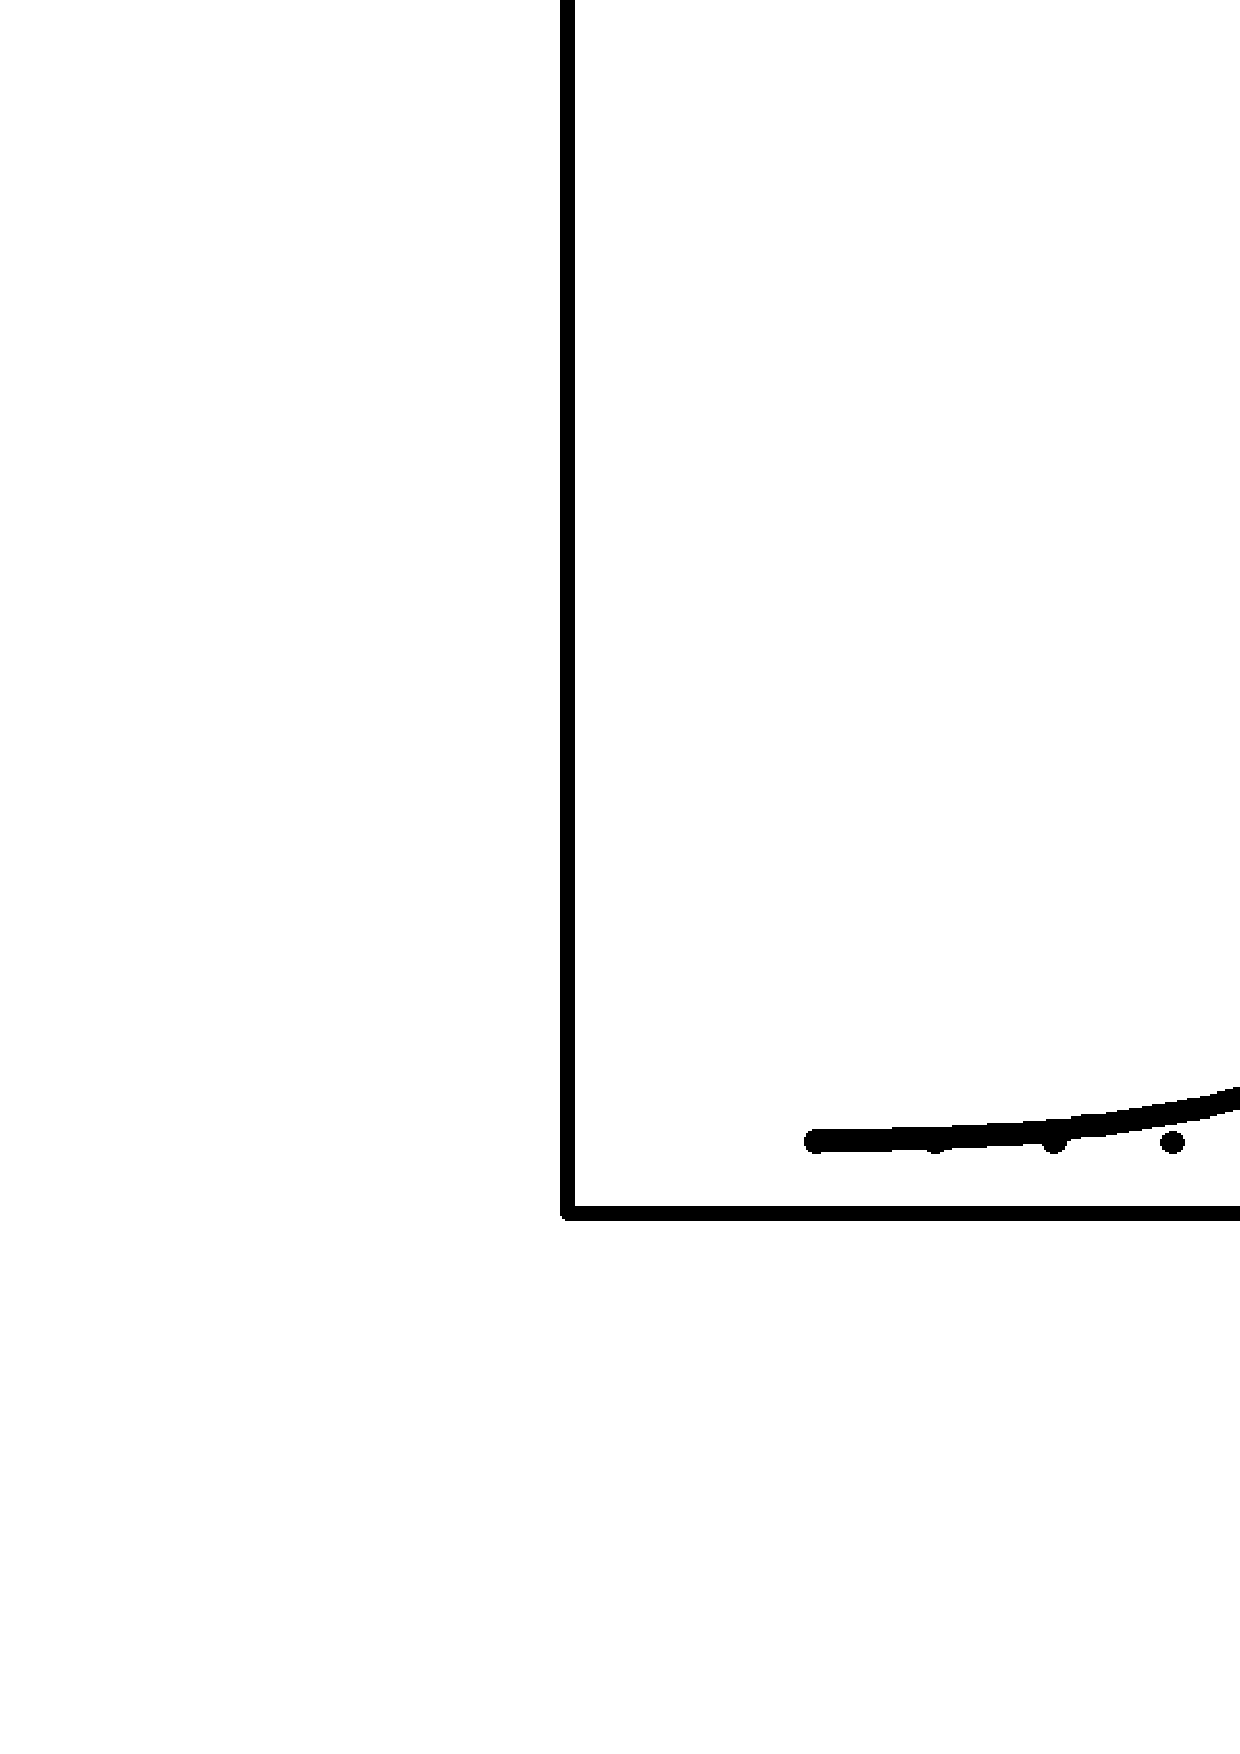
\includegraphics[width=0.88\textwidth]{Fig4_2}
\vspace{-3mm}
\caption{Температурний режим (верхні залежності) та
відповідні сигнали термостимульваного струму (нижні)
за наявності двох рівнів.}
\vspace{-3mm}
\label{F42}
\end{figure}


\chapter{Магніто--резонансні методи}\label{chapER}

Для дослідження дефектів широко використовують
методи електронного парамагнітного резонансу
(electron paramagnetic resonance, EPR) та подвійного електронно--ядерного резонансу
(electron nuclear double resonance, ENDOR).

EPR полягає у дослідженні резонансного поглинання електромагнітного випромінювання неспареними
електронами або системою неспарених електронів у магнітному полі.
При внесенні атома у зовнішнє магнітне поле буде
останнє буде взаємодіяти з орбітальним та спіновими магнітними моментами
неспарених електронів, а також впливати на спін--орбітальну взаємодію.
У спрощеному випадку оператор збурень, який описує ці ефекти виглядатиме наступним чином
\begin{equation}
\hat{H}_B=-(\hat{\vec{\mu}}_L+\hat{\vec{\mu}}_S)\cdot\vec{B}+A_{LS}\hat{\vec{L}}\cdot\hat{\vec{S}}\,,
\end{equation}
де
$\vec{B}$ --- вектор індукції зовнішнього магнітного поля,
$\hat{\vec{\mu}}_L=-\frac{q}{2m_0}\hat{\vec{L}}$ та
$\hat{\vec{\mu}}_S=-\frac{qg_0}{2m_0}\hat{\vec{S}}$
--- оператори повних магнітних моментів, пов'язаних з орбітальним рухом та спіном,
відповідно;
$\hat{\vec{L}}$ та $\hat{\vec{S}}$--- оператори повних орбітального та спінового моментів атому, відповідно;
$A_{LS}$ --- стала спін--орбітальної взаємодії,
$g_0\!\approx\!2$ --- гіромагнітний фактор.
Знехтувавши діамагнітною та спін-спіновою взаємодіями оператор можна записати у
вигляді \cite{tuomisto2019}
\begin{equation}
\hat{H}_B=\frac{q}{2m_0}\vec{B}\cdot\tilde{g}\cdot\hat{\vec{S}}\,,
\end{equation}
де компоненти g--тензора (або тензора Ланде) залежать від стану
атома та в $n$-му з них визначаються наступним чином
\begin{equation}
\tilde{g}_{ij}=g_0\,\delta_{ij}-2A_{LS}\sum_{m\neq n}\frac{\langle\psi_n\mid\hat{L}_i\mid\psi_m\rangle
\langle\psi_m\mid\hat{L}_j\mid\psi_n\rangle}{E_m-E_n}\,,
\end{equation}
де
$\delta_{ij}$ --- символ Кронекера, а
$\psi_n$ та $E_n$ --- власні функції та власні значення незбуреного гамільтоніана.
Тобто, у кристалічній ґратці звичайний $g_0$ стає тензором другого рангу.
Відхилення його діагональних компонент  від $g_0$ пов'язане з впливом
збуджених станів на основний внаслідок спін--орбітальної взаємодії.
Власні значення та напрямки тензора $\tilde{g}$ віддзеркалюють
властивості локальної симетрії парамагнітного дефекту і дозволяють отримать
важливу інформацію щодо розташування оточуючих атомів.



Отже, для системи (дефекту) з наявністю неспарених електронів,
тобто з парамагнітними властивостями, в зовнішньому магнітному полі
буде спостерігатися розщеплення енергетичного рівня на декілька,
кожному з яких відповідатиме свій стан (орієнтація)
магнітного моменту.
Якщо традиційно спрямувати вісь $Z$ за напрямком магнітного поля і
врахувати, що власні значення $z$--ої компоненти оператора повного спіну
мають вигляд $S_z=\hbar m_S$
(де $m_S$ --- спінове магнітне число), то величина зсуву енергії кожного з підрівнів може бути записана у вигляді
\begin{equation}
\Delta E_B=\tilde{g}\,m_s\, \mu_B\,B\,,
\end{equation}
де
$\mu_B=\frac{q\hbar}{2m_0}$ --- магнетон Бора.
Внаслідок тензорних властивостей $\tilde{g}$ розщеплення енергетичних
рівнів стає анізотропним.

\begin{figure}[!b]
\center
\vspace{-5mm}
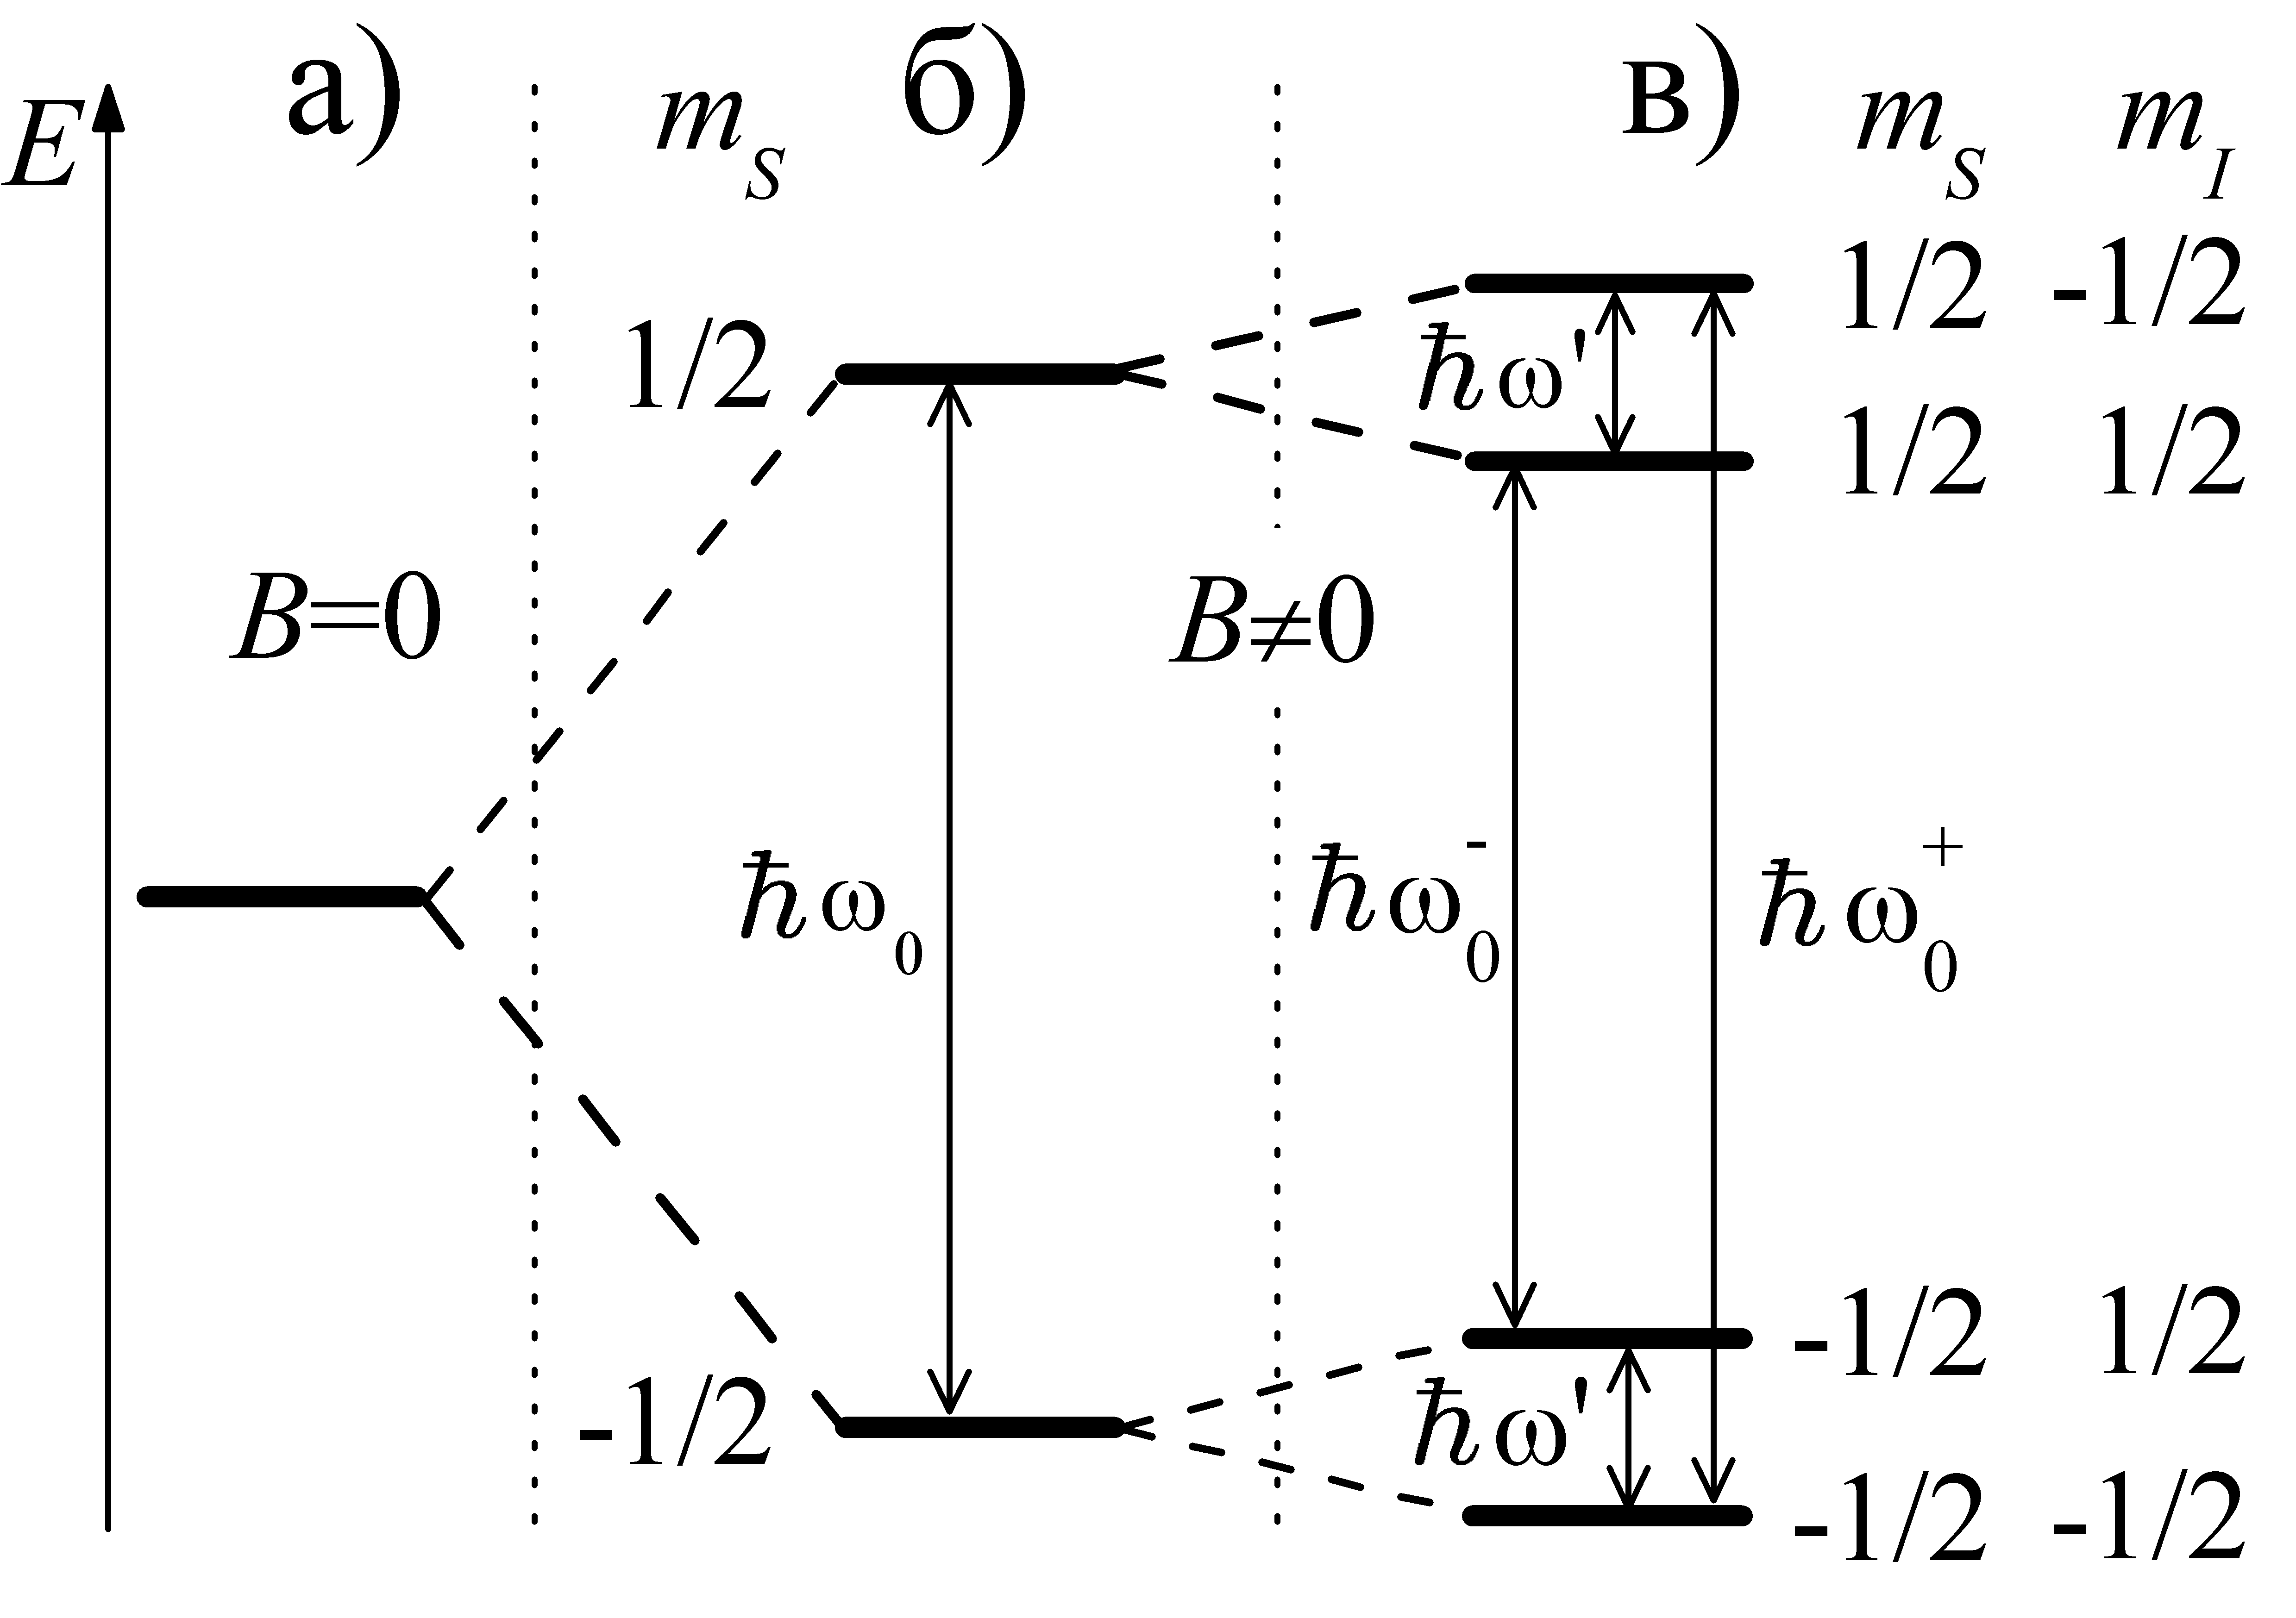
\includegraphics[width=0.65\textwidth]{Fig5_1}
\vspace{-3mm}
\caption{Розщеплення рівнів парамагнітного дефекту зі спіном $S=\frac{1}{2}$
без (б) та з (в) врахуванням надтонкої взаємодії з ядром, для якого  $I=\frac{1}{2}$.
Для частини (а) вважається, що зовнішнє магнітне поле відсутнє.
Стрілки вказують дозволені переходи.
}
\vspace{-3mm}
\label{F51}
\end{figure}

На рис.~\ref{F51},б показана схема зняття виродження у найпростішому випадку.
Між розщепленими рівнями можуть відбуватися переходи, ініційовані
електромагнітним випромінюванням, причому
поглинатися будуть лише хвилі з частотою $\omega_0$,
яка відповідає різниці енергій між станами.
Тобто, між станами, утвореними за рахунок прикладання магнітного поля можуть
проходити резонансні переходи.
Враховуючи, що правило відбору у дипольному наближенні виглядає $\Delta m_S=\pm1$,
то для частоти, на якій спостерігається поглинання, справедливим буде наступне співвідношення
\begin{equation}
\hbar\omega_0=\tilde{g}\, \mu_B\,B\,,
\end{equation}
тобто вона залежить як від величини магнітного моменту, так і від індукції магнітного поля.
В лабораторних умовах найчастіше використовують поля в околі $(0,1\div1)$~Тл ($(10^3\div10^4)$~Гс),
яким
відповідає
%при $\tilde{g}=2$ відповідатиме $\omega_0=(3\div30)$~ГГц, тобто мова йде про
мікрохвильовий або далекий інфрачервоний діапазон.

\begin{figure}[!b]
\center
\vspace{-5mm}
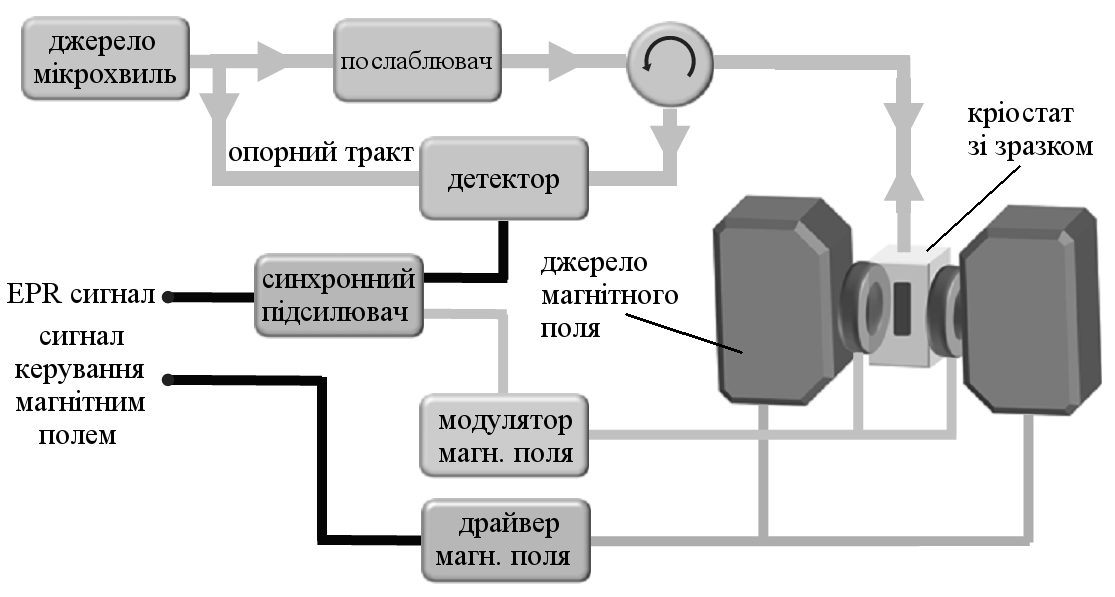
\includegraphics[width=0.95\textwidth]{Fig5_2}
\vspace{-3mm}
\caption{Схема типової установки для EPR вимірювань.
Рисунок адаптовано з \cite{tuomisto2019}.
}
\vspace{-3mm}
\label{F52}
\end{figure}



Експериментально проводиться вимірювання поглинутої потужності $P_{abs}$
електромагнітної хвилі.
Схема типової установки наведена на рис.~\ref{F52}.
Поглинання енергії пов'язано зі зміною магнітного моменту атому,
яка, в свою чергу, спричинює зміну магнітної сприйнятливості $\chi$.
Загалом $\chi=\chi\prime+i\chi\prime\prime$,
де $\chi\prime$ визначає розсіяння, а $\chi\prime\prime$ --- поглинання:
\begin{equation}\label{EPRP}
P_{abs}(\omega)=\omega\,B_1^2\,\chi\prime\prime=\frac{\omega\,B_1^2}{2}\cdot\frac{\gamma_{i} J_0 \tau_{r,2}}
 {1+(\omega-\omega_0)^2\tau_{r,2}^2+\gamma^2B_1^2\tau_{r,1}\tau_{r,2}}\,,
\end{equation}
де
$B_1$ --- індукція радіочастотного поля;
$\gamma_{i}$ --- гіромагнітне співвідношення;
$J_0$ --- намагніченість; якщо вона пов'язана з парамагнітними дефектами, то
\begin{equation}\label{EPRJ0}
J_0=\frac{\tilde{g}^2\mu_B^2N_t\,S(S+1)}{3kT}\,B\,,
\end{equation}
$\tau_{r,1}$ --- спін--ґратковий або повздовжній час релаксації,
характеризує обмін енергії між парамагнітними спінами та тепловими
коливаннями оточуючих атомів (характерний час зникнення намагніченості
після вимкнення зовнішнього магнітного поля);
$\tau_{r,2}$ --- спін--спіновий або поперечний час релаксації,
пов'язаний зі взаємодією спінів при зміні зовнішнього поля
(характерний час зникнення упорядкованості прецесії різних магнітних моментів
під дією $B_1$ після його вимкнення).
При $\gamma^2B_1^2\tau_{r,1}\tau_{r,2}\ll 1$ частотна залежність поглинутої
потужності описується функцією Лоренця --- див. рис.~\ref{F53},а.


\begin{figure}[!t]
\center
\vspace{-5mm}
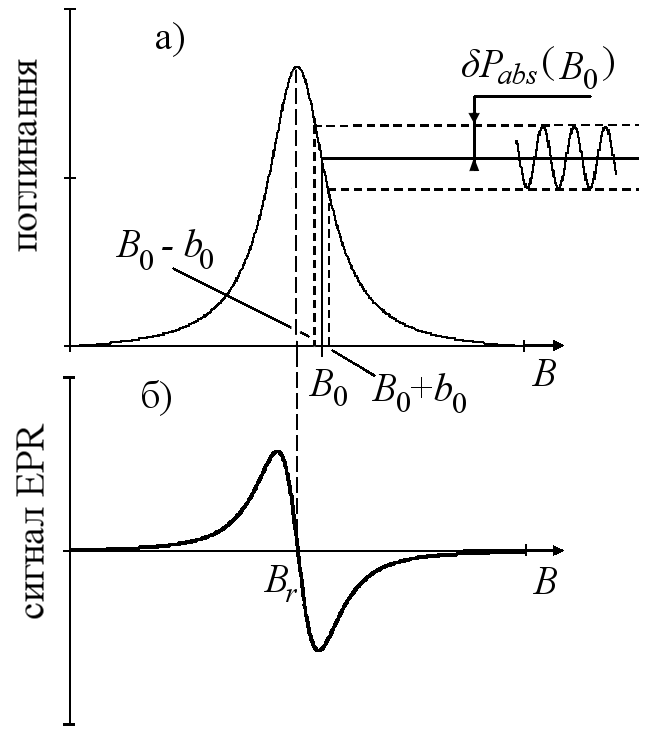
\includegraphics[width=0.65\textwidth]{Fig5_3}
\vspace{-3mm}
\caption{Форма лінії поглинання (а) та сигналу EPR (б).
}
\vspace{-3mm}
\label{F53}
\end{figure}

Загалом, існує два способи отримання резонансного поглинання при EPR:
а)~зміна частоти мікрохвильового випромінювання при постійному полі;
б)~зміна величини індукції поля (а отже і $\omega_0$) при фіксованому значенні $\omega$.
Проте через те, що потужність джерел мікрохвильового випромінювання суттєво залежить
від частоти та через інші технічні причини на практиці використовується саме другий підхід.
Типові частоти мікрохвильового випромінення та назви відповідних ліній наведено у Таблиці~\ref{tablEPR}.


\begin{table}[!t]
\caption {Типові частоти мікрохвильового випромінювання, що використовуються в EPR.}
\label{tablEPR}
\vspace{-3mm}%\center{
\begin{tabularx}{\textwidth}{|>{\centering\arraybackslash}X|>{\centering\arraybackslash}X|>{\centering\arraybackslash}X|>{\centering\arraybackslash}X|}
  \hline
  Назва смуги & Частота, ГГц&Довжина хвилі, см &Резонансне магнітне поле$^*$, мТл    \tabularnewline \hline
 L &1,2& 30& 43 \tabularnewline \hline
S &3,6& 8,3& 128\tabularnewline \hline
X& 9,5& 3,2& 339\tabularnewline \hline
K &24 &1,25& 856\tabularnewline \hline
Q& 35& 0,85& 1250\tabularnewline \hline
W &94 &0,32 &3354\tabularnewline \hline
G &180 &0,17 &6423\tabularnewline \hline
\multicolumn{4}{l}{$^*$ \emph{при} $\tilde{g}=2$}\tabularnewline
\end{tabularx}
%\end{tabular}
%}
\end{table}
%\vspace{-3mm}

Крім того, з метою підвищення чутливості,
на постійне зовнішнє поле накладається змінне гармонічне з амплітудою $b_0$ та частотою близько 100~кГц.
Частота такої модуляції має бути повільною порівняно з часом релаксації,
так як система повинна залишатися в тепловій рівновазі при проходженні через резонанс.
Тобто, для заданого статичного значення $B_0$ зовнішнє поле у зразку змінюється
від $(B_0-b_0)$ до $(B_0+b_0)$,
а поглинання осцилює з амплітудою $\delta P_{abs}(B_0)$, яка
пропорційна нахилу лінії поглинання при даній величині індукції --- див рис.~\ref{F53},a.
Синхронний підсилювач у схемі реєстрації фільтрує
коливання та дозволяє отримати сигнал,
який є першою похідною лінії поглинання за магнітним полем.
Відповідна форма сигналу EPR показана на рис.~\ref{F53},б.
При резонансі $\delta P_{abs}(B_r)=0$, а отже і сигнал EPR проходить через нуль.
Відповідно, форма лінії резонансу EPR описується похідною від функції Лоренця.
Якщо присутнє неоднорідне розширення, то
лінія має профіль Фойгта: згортка ліній Гауса та Лоренця.

З виразів (\ref{EPRJ0}) та (\ref{EPRP}), амплітуда поглинання
обернено пропорційна температурі.
Як наслідок --- вимірювання найчастіше проводять при зниженій температурі.
Якщо основний стан дефекту, на відміну від збудженого, не парамагнітний,
то для реалізації можливості спостереження сигналу EPR нерідко використовується оптичне збудження.

EPR вимірювання дозволяють отримати наступну інформацію:
\begin{enumerate}[label=\asbuk*),leftmargin=0em,itemindent=1.5em]
%\begin{enumerate}[label=\arabic*),leftmargin=0em,itemindent=1.5em]
\item сам факт спостереження спектру свідчить про те, що центр парамагнітний;
 зворотній висновок не завжди справедливий, так як може реалізовуватися ситуація, коли концентрація
 дефектів просто недостатня для реєстрації сигналу;
\item площа під спектром поглинання пов'язана з числом магнітних моментів,
а отже базуючись на цю величину можна визначити концентрацію дефектів;
\item положення резонансу у спектрі поглинання однозначно пов'язане з частотою
та індукцією магнітного поля і це дозволяє визначити ефективний магнітний момент і
величину $\tilde{g}$--фактора;
\item залежність резонансної частоти ($\tilde{g}$--фактора) від кута між зовнішнім полем та віссю симетрії
кристалу віддзеркалює локальну симетрію дефекту;
загалом, EPR є чи не найчутливішим методом дослідження відхилення від загальної
симетрії та дозволяє розрізнити навіть такі відхилення, що
не можуть бути виявлені за допомогою рентгеноструктурного аналізу;
\item можна досліджувати
зворотні та незворотні динамічні процеси збудження,
перетворення, виникнення та дифузії дефектів;
зокрема аналіз температурних залежностей спектрів дозволяє
визначити енергію активації цих процесів;
\item кількість ліній у надтонкій структурі спектрів дозволяє
оцінити кількість і тип ядер, пов'язаних з дефектом;
величина розщеплення у надтонкій структурі пов'язана з електронною густиною
в околі дефекту, а її анізотропія віддзеркалює анізотропію цієї густини та локальну
симетрію дефекту.
\end{enumerate}

Зупинимось на останньому детальніше.
Надтонка структура виникає внаслідок взаємодії електронів
з магнітним (або електричним квадрупольним) моментом ядра (або ядер) самого
дефекту чи й  оточуючих його ядер ґратки.
В останньому випадку нерідко використовується термін супернадтонка структура.
Взаємодія описується оператором
\begin{equation}
\hat{H}_{SI}=\sum_j\hat{\vec{S}}\cdot\tilde{A}_j\cdot\hat{\vec{I}}_j\,,
\end{equation}
де сумування відбувається по ядрам, що приймають участь у взаємодії,
$\hat{\vec{I}}_j$ --- оператор спіну $n$--го ядра,
$\tilde{A}_j$ --- симетричний тензор надтонкої взаємодії.
Взаємодія викликає додаткове розщеплення енергетичних рівнів у магнітному полі
(див. рис.~\ref{F51},в).
При його розгляді необхідно врахувати, що
спектр оператора $\hat{\vec{I}}$ схожий до спектрів інших операторів моментів,
зокрема проекція на вісь $Z$ дорівнює $\hbar m_I$,
де $m_I$ --- ядерне магнітне число.
При переходах має виконуватися правило відбору $\Delta m_I=0$.

Надтонка взаємодія дає інформацію про хімічну природу дефекту,
так як величина ядерного спіну є специфічною характеристикою атому.
Зокрема, вміст взаємодіючих ядер може бути визначений
зі співвідношення інтенсивностей надтонких ліній та центральним резонансом.
Супернадтонка взаємодія віддзеркалює локальну симетрію хвильової функції поблизу
взаємодіючих ядер, а отже визначення власних значень та власних
напрямків тензору $\tilde{A}$ ядер найближчого оточення дає додаткову інформацію
про його симетрію, що дозволяє більш точно визначити мікроструктуру
парамагнітного дефекту.

Лінії надтонкої структури, що виникає внаслідок взаємодії з власним ядром,
розрізняються у звичайному EPR, тоді як супернадтонка структура у більшості
випадків проявляється лише у неоднорідному уширенні ліній.
Більш детальну інформація про супернадтонку структуру зокрема можна отримати
у методі подвійного електронно--ядерного резонансу, де саме і
досліджуються переходи між енергетичними рівнями, які виникли внаслідок взаємодії з ядром.

У ENDOR для виявлення ядерних резонансних переходів використовується сигнал EPR.
А саме, спостерігається часткове відновлення попередньо насиченого EPR переходу.
Для цього зовнішнє магнітне поле фіксують на величині, яка
відповідає резонансу, і збільшують інтенсивність мікрохвильового випромінювання з енергією $\hbar\omega_0^+$ (рис.~\ref{F51},в).
Якщо відповідний перехід здійснить переважна кількість електронів,
то EPR сигнал послабиться.
Після цього накладають додаткове випромінювання
зі змінною частотою.
Коли енергія цього радіочастотного електромагнітного поля стає рівною $\hbar \omega'$,
заселеність рівнів змінюється --- наприклад
зменшується заселеність рівня з $m_S\!=\!+1/2$ та $m_I\!=\!+1/2$ внаслідок
резонансного випромінювання.
При цьому EPR--перехід перестає бути насиченим і поглинання зростає.
Спектр ENDOR --- це залежність інтенсивності EPR сигналу від частоти додаткового
опромінювання.

На відміну від EPR, ENDOR не є кількісним методом,
так як інтенсивність його спектральних ліній залежить від багатьох
механізмів релаксації в системі електронів та ядер.
Як наслідок --- ні кількість ядер, які беруть участь у надтонкій взаємодії,
ні величина їхнього спіну не можуть бути визначено безпосередньо.
Проте вони можуть бути однозначно ідентифіковані за величиною ядерного $\tilde{g}$--фактора,
який вимірюється в ENDOR.
Чутливість ENDOR складає декілька відсотків відносно чутливості EPR.
Збільшення концентрації дефектів, з одного боку, ніби є бажаним з точки зору збільшення інтенсивності сигналу,
проте, з іншого, може викликати  появу дипольної взаємодії та (або) механізмів обміну,
що зменшують час релаксації $\tau_{r,2}$ та призводять до розширення резонансної лінї;
як наслідок, насичення стає неможливим і сигнал не виявляється взагалі.